\begin{tcolorbox}[
    enhanced,                   % Required for borderline drawing
    boxrule=0pt,                % Hide default uniform frame
    colback=white,              % Background color (set as needed)
    % Top: teal, 2.5pt
    borderline north={1.5pt}{-1.5pt}{black},
    % Bottom: different color, 0.5pt
    borderline south={3.0pt}{-3.0pt}{povteal},
    leftrule=0pt,       % No left line
    rightrule=0pt,      % No right line
    top=0pt,
    bottom=0pt,
    left=4pt,
    right=6pt,
    boxsep=0pt,         % Matches mdframed inner margins behavior
    arc=0pt,
  ]
  \begin{tblr}{
      colspec = { Q[c, m, wd=2.4cm] Q[c, m, wd = .65\textwidth] Q[c, m, wd=3.15cm] },
      colsep  = 4pt,
      rowsep  = 0pt,
      column{2} = {bg=gray!20},
    }

    %--- LEFT: ITC Logo ---
    {
      \parbox{2.2cm}{%
        \centering
        \includegraphics*[width=2.2cm]{Logo/ITC}
      }
    }
    &

    %--- CENTER: Journal Title ---
    {
      \centering
      \vspace*{.2cm}

      {\fontsize{14}{22}\selectfont\textbf{THE $15^{\textbf{TH}}$ SCIENTIFIC DAY OF ITC}}\par
      \vspace{.4cm}
      {\fontsize{14}{22}\selectfont Bridging Engineering and Technology with Industry for Cambodia’s Sustainable Growth}

      \vspace*{.2cm}
    }
    &

    %--- RIGHT: RIC Logo ---
    {
      \parbox{3cm}{%
        \centering
        \includegraphics*[width=3cm]{Logo/RIC}
      }
    }
  \end{tblr}
\end{tcolorbox}

% ─── Title block ──────────────────────────────────────────────────────────────
\vspace{0.1in}
\begin{center}
  {\fontsize{14}{22}\selectfont\textbf{Efficient Attention Classification: A Lightweight XGBoost Approach to Facial Feature Extraction in E-Learning}}\\[9pt]

  {\fontsize{12}{22}
    Hengborann MOUL\textsuperscript{\color{superscript}\hyperlink{aff1}{\color{superscript} 1*}},\;
    Dr. Sothea HAS\textsuperscript{\color{superscript}\hyperlink{aff2}{\color{superscript} 2}},\;
    Dr. Sokkhey PHAUK\textsuperscript{\color{superscript}\hyperlink{aff2}{\color{superscript} 2}}\\[6pt]
  }

  \textit{
    \textsuperscript{\hypertarget{aff1}{\color{superscript}1}}Graduate School, Institute of Technology of Cambodia, Russian Federation Blvd., P.O. Box 86, Phnom Penh, Cambodia
  }\\[7pt]
  \textit{
    \textsuperscript{\hypertarget{aff2}{\color{superscript}2}}Department of Applied Mathematics and Statistics, Institute of Technology of Cambodia, Russian Federation Blvd., P.O. Box 86, Phnom Penh, Cambodia
  }\\[7pt]

  {\textsuperscript{\color{superscript}\hyperlink{aff1}{\color{superscript} *}}Corresponding author: \href{mailto:hengborann_moul@gsc.itc.edu.kh}{%
    \textcolor{povteal}{hengborann\_moul@gsc.itc.edu.kh}%
  }}
\end{center}

\vspace{5pt}

% ─── Abstract ─────────────────────────────────────────────────────────────────
\begin{mdframed}[
    innerleftmargin=5pt,
    innerrightmargin=7pt,
    innertopmargin=6pt,
    innerbottommargin=6pt,
    topline=false,
    bottomline=false,
    skipabove=5pt,
    skipbelow=5pt,
    leftline=false,
    rightline=false,
  ]
  \noindent\textbf{Abstract:}
  \textit{
    The COVID-19 pandemic moved education online overnight, and with that shift came a problem technology alone did not solve. In a physical classroom, disengagement has visible signals: a student who stopped writing, one staring past the screen, one who has gone quiet. Those signals disappear on a video call. Existing automated detection systems try to recover them but lean on deep learning pipelines that need hardware most schools do not have, and nearly all reduce engagement to a flat binary that ignores how gradually attention fades. This study uses the DAiSEE benchmark, a standard collection for in-the-wild student engagement recognition covering four affective states: boredom, engagement, confusion, and frustration, each classified at three ordinal levels: Low, Medium, and High. Per frame, 78 features are extracted through computer vision covering facial landmarks, head pose, eye gaze, and action unit intensities, then passed into an XGBoost classifier. Beyond predictions, XGBoost outputs feature important scores that identify which facial cues most influence each decision, making the model transparent in a way neural networks typically are not. The model achieves a mean accuracy of 65.26\% and a weighted F1-score of 59.62\%, with frustration reaching 80.25\% per-class accuracy. Macro F1 sits at 0.397, pulled down by DAiSEE's class imbalance and the difficulty of separating Mid-level states, a challenge deep learning baselines on this dataset also struggle with. Feature importance analysis reveals that AU-based features account for 60\% of the top-20 ranked features, confirming that facial muscle activity carries more predictive signal than head pose or gaze alone. The full pipeline runs without GPU acceleration, making it deployable on standard classroom hardware. This work contributes toward SDG4 Quality Education by giving educators a practical, explainable attention detection tool for data-driven teaching in resource-constrained online learning environments where disengagement often goes unnoticed.
  }
\end{mdframed}

\vspace*{-8pt}

\begin{mdframed}[
    linecolor=povteal,
    linewidth=.4pt,
    topline=false,
    bottomline=false,
    leftline=false,
    rightline=false,
    innertopmargin=6pt,
    innerbottommargin=6pt,
    innerleftmargin=6pt,
    innerrightmargin=6pt,
  ]
  \noindent\textbf{Keywords:}
  Student Engagement Detection; Affective State Classification; Feature Extraction; Extreme Gradient Boosting (XGBoost); Computer Vision
\end{mdframed}

\vspace{9pt}

% ─── Two-column body ──────────────────────────────────────────────────────────
\setlength{\columnsep}{.7cm} % space between columns
\begin{multicols}{2}
  \setlength{\parindent}{1em}
  \setlength{\parskip}{8pt}

  % ─────────────────────────────────────────────────────────────────────────────
  \section{Introduction}

  % ───── Corresponding author ─────────────────────────────────────────────────────
  \renewcommand{\thefootnote}{}
  \footnotetext{
    \color{superscript}\hyperlink{aff1}{\color{superscript}$^{*}$} Corresponding author: Hengborann MOUL.\\
    \hspace*{.65cm}
    \textit{E-mail: \href{mailto:hengborann_moul@gsc.itc.edu.kh}{hengborann\_moul@gsc.itc.edu.kh}; Tel: +855-11~836~711}.
  }
  \renewcommand{\thefootnote}{\arabic{footnote}}
  ~~~
  The rapid pivot to online education during the COVID-19 pandemic did more than move lectures to video calls. It quietly erased one of teaching's most powerful tools: the ability to read the room. In a physical classroom, a teacher instantly registers the subtle signals of disengagement, a student who stops scribbling notes, stares blankly past the screen, or falls silent. Those cues vanish in remote settings, leaving educators navigating virtual silence without the real-time feedback that has guided effective instruction for generations~\cite{prakasha2023student, Hollister2022EngagementIO}.

  This loss matters. Student engagement is not a binary switch between paying attention and checked out. It unfolds gradually across nuanced affective states, boredom that creeps in, confusion that builds, frustration that spikes, or the quiet flow of genuine engagement~\cite{Gupta2016DAiSEETU}. Yet most automated detection systems developed for online classrooms rely on heavyweight deep-learning pipelines that demand GPU resources most schools simply cannot afford~\cite{Zhang2019AnNE, Su2024LeveragingPA, Khenkar2023DeepAO}. Even when they work, they often collapse these rich emotional gradients into a flat engaged or disengaged label, missing the very gradations educators need for timely, targeted intervention~\cite{Santoni2023ConvolutionalNN, Malekshahi2024AGM}.

  While deep-learning models have pushed the frontier of affective-state recognition on in-the-wild benchmarks such as DAiSEE~\cite{Gupta2016DAiSEETU}, the literature still lacks a practical, transparent alternative that runs on everyday classroom hardware and explains why it makes each decision~\cite{Khosravi2022ExplainableAI, CortiasLorenzo2023TowardEA}. Hand-engineered computer-vision features paired with classical gradient boosting have been underexplored for this multi-level, multi-class problem, despite their proven efficiency and interpretability in other domains~\cite{Hossen2023AttentionMO, Das2025OptimizingSE}.

  To close this gap, we introduce a lightweight framework that extracts a compact 78-dimensional feature vector, capturing facial landmarks, head-pose orientation, eye-gaze direction, and facial-action-unit intensities, from each video frame and feeds it directly into an XGBoost classifier~\cite{Chen2016XGBoostAS}. The model operates entirely on CPU, delivers per-frame predictions across four affective states (boredom, engagement, confusion, frustration) at three ordinal levels (Low, Medium, High), and surfaces feature-importance scores that reveal exactly which facial cues drive each classification.

  Our objective is straightforward yet ambitious: demonstrate that principled feature engineering combined with gradient boosting can achieve competitive performance on the DAiSEE benchmark while remaining fully explainable and deployable at scale. The resulting system attains 65.26\% mean accuracy and 59.62\% weighted F1-score, with frustration detection reaching 80.25\% per-class accuracy, results that rival far more resource-intensive deep-learning baselines yet run without specialized hardware and offer educators human-interpretable insights~\cite{Das2025OptimizingSE}.

  This work matters because it equips teachers with a practical, data-driven window into student attention that fits existing classroom infrastructure. By making disengagement visible again and explainable, we enable timely instructional adjustments that can improve learning outcomes at population scale~\cite{Khosravi2022ExplainableAI}.

  % ------------ End Introduction ----------- %

  % ─────────────────────────────────────────────────────────────────────────────
  \begin{comment}
  \section{Literature Review}
  ~~~
  Since its public release in 2016, the DAiSEE dataset has become the de facto benchmark for affective-state recognition in e-learning environments. Gupta and colleagues~\cite{Gupta2016DAiSEETU} created this in-the-wild collection of 9068 ten-second video clips from 112 participants, annotated for four states (boredom, engagement, confusion, and frustration) each at four ordinal levels. The original paper already established baseline performance using standard video-classification networks, yet those early results hovered around 40 percent accuracy and highlighted the inherent difficulty of the multi-class, multi-level problem.

  Subsequent research has overwhelmingly turned to deep-learning architectures to push performance higher. Zhang and co-authors in 2019~\cite{Zhang2019AnNE} introduced one of the first end-to-end convolutional networks tailored for DAiSEE, reporting strong binary engaged-versus-disengaged accuracy while still struggling with the finer ordinal distinctions. Jiang followed in 2021~\cite{jiang2021engagement} with a comparative study of several convolutional backbones, confirming that temporal modeling helps but at the cost of increased computational demand. Solanki and Mandal in 2022~\cite{Solanki2022EngagementAU} presented a multi-level classification approach that recorded testing accuracies up to 86.6 percent for certain affective states, further underscoring the value of treating labels as ordered rather than purely categorical.

  By 2022, transformer-based and attention-driven methods began to appear. Yang and colleagues proposed an attention-based video classification framework for engagement recognition~\cite{Yang2022AttentionbasedVC}, while Komaravalli and co-workers in 2023~\cite{Komaravalli2023DetectingAA} created a customized single-label version of DAiSEE to improve frame-level affective-state detection. In the same year, several groups explored hybrid and resource-aware designs. Khenkar et al.~\cite{Khenkar2023DeepAO} developed 3D-CNN models that explicitly incorporated body activity alongside facial cues, while Santoni and colleagues~\cite{Santoni2023ConvolutionalNN} focused on handling DAiSEE's severe class imbalance through specialized CNN training strategies. Around the same time, Hossen and Uddin~\cite{Hossen2023AttentionMO} demonstrated that classical gradient-boosting machines fed with OpenFace features could reach surprisingly high attentiveness detection rates, hinting at the potential of lighter pipelines.

  More recent 2024 contributions have continued to refine deep architectures. Su and co-authors~\cite{Su2024LeveragingPA} presented a hybrid DTransformer that combines part-and-sensitive attention with spatiotemporal transformers, attaining 64 percent test accuracy on DAiSEE. Malekshahi et al.~\cite{Malekshahi2024AGM} introduced a general lightweight model that preserves temporal relationships across frames and achieved 68.57 percent accuracy through careful label adaptation, yet still relied on GPU acceleration for training. Khan and Safa~\cite{Khan2024RevisitingAI} revisited the original annotations, providing expert-validated re-annotations that highlight ongoing challenges with label quality and consistency.

  Across this body of work (more than ten distinct DAiSEE-based studies spanning 2016 to 2024), two consistent limitations emerge. First, nearly all high-performing models depend on deep convolutional or transformer backbones that require GPU resources unavailable in most school environments. Second, the black-box nature of these networks offers little insight into which facial cues drive predictions, making it hard for educators to trust or debug the system in real time. Hand-engineered features paired with interpretable boosters such as XGBoost remain underexplored for the full four-state, three-level DAiSEE task, despite their proven efficiency and transparency in related domains.

  Our work directly addresses these gaps by extracting a compact 78-dimensional computer-vision feature set and feeding it directly into an XGBoost classifier. In doing so, we provide both competitive performance and per-prediction explanations without any specialized hardware, offering a practical and educator-friendly alternative to the deep-learning mainstream.

  \end{comment}

  % ─────────────────────────────────────────────────────────────────────────────
  \section{Methodology}
  \subsection{Dataset}
  \subsubsection{DAiSEE Dataset}

  This study employs the DAiSEE (Dataset for Affective States in E-Environments) dataset, a large-scale benchmark for affective state recognition in online learning contexts\cite{Gupta2016DAiSEETU}. The dataset comprises video recordings of students engaged with online educational content. The DAiSEE dataset provides annotations for four distinct affective states: boredom, engagement, confusion, and frustration. Each affective state is annotated using a four-level ordinal scale (Very Low = 0, Low = 1, High = 2, Very High = 3) based on crowd-sourced annotations from multiple raters.

  \begin{table}[H]
    \caption{\footnotesize{Distribution of labels in DAiSEE across its affective states}}
    \label{tab_daisee_labels}
    \centering
    \begin{tabular}{c>{\small}c>{\small}c>{\small}c>{\small}c}
      \hline
      \textbf{Affective State} & \textbf{Very Low} & \textbf{Low}  & \textbf{High} & \textbf{Very High} \\ \hline
      Boredom         & 3869     & 2931 & \cellcolor{gray!20}{1934} & \cellcolor{gray!20}{334}       \\ \hline
      Confusion       & 6024     & 2191 & \cellcolor{gray!20}{752}  & \cellcolor{gray!20}{101}       \\ \hline
      Engagement      & \cellcolor{gray!20}{61}       & \cellcolor{gray!20}{459}  & 4477 & 4071      \\ \hline
      Frustration     & 6986     & 1649 & \cellcolor{gray!20}{346}  & \cellcolor{gray!20}{87}        \\ \hline
    \end{tabular}
  \end{table}

  The dataset contains video clips of varying durations, captured at 30 frames per second, with participants from diverse demographic backgrounds. The videos capture naturalistic student behavior during online learning sessions, providing authentic expressions of affective states. The original dataset is organized into training, validation, and test splits, with label files containing the ground truth annotations for each video clip.

  % The distribution of labels after removing bad annotators is depicted in Table~\ref{tab_daisee_labels}

  \subsubsection{Label Transformation}

  The original DAiSEE dataset provides four-level labels for each affective state. However, empirical analysis of the dataset reveals significant class imbalance, particularly the extreme scarcity of samples in the ``Very High'' category for several affective states. Furthermore, distinguishing between adjacent levels (e.g., ``High'' versus ``Very High'') presents substantial challenges even for human annotators, potentially introducing noise into the training process.

  To address these challenges while maintaining clinically meaningful distinctions, we collapse the four-level labels into a three-level classification scheme. The transformation strategy is state-specific and informed by the psychological characteristics of each affective construct:

  \begin{itemize}
    \item \textbf{Boredom, Confusion, and Frustration:} These states follow a similar remapping where levels 0 (Very Low), 1 (Low), and 2 (High) remain unchanged, while level 3 (Very High) is merged into level 2. This consolidation is justified by the observation that extreme manifestations of these negative affective states are rare in educational contexts, and the distinction between ``High'' and ``Very High'' levels provides limited additional discriminative value for automated recognition systems.

    \item \textbf{Engagement:} Following a distinct remapping strategy, levels 0 (Very Low) and 1 (Low) are merged into a single ``Low'' category (mapped to 0), level 2 (High) is mapped to 1, and level 3 (Very High) is mapped to 2. This transformation reflects the practical reality that distinguishing between minimal and moderate disengagement is less critical than identifying high engagement states, which are of primary pedagogical interest.
  \end{itemize}

  Mathematically, the label transformation functions are defined as:

  For $s \in \{\text{boredom}, \text{confusion}, \text{frustration}\}$:
  \begin{equation}
    y'_s =
    \begin{cases}
      y_s & \text{if } y_s \in \{0, 1\} \\
      2 & \text{if } y_s \in \{2, 3\}
    \end{cases}
  \end{equation}

  For engagement:
  \begin{equation}
    y'_{\text{engagement}} =
    \begin{cases}
      0 & \text{if } y_{\text{engagement}} \in \{0, 1\} \\
      1 & \text{if } y_{\text{engagement}} = 2 \\
      2 & \text{if } y_{\text{engagement}} = 3
    \end{cases}
  \end{equation}

  \noindent where $y_s$ represents the original four-level label and $y'_s$ denotes the transformed three-level label for affective state $s$.

  \subsection{Data Preprocessing}
  The entire process start with the preprocessing of DAiSEE datasets. Each video of DAiSEE was chunk and extracted facial features from each frame. Following in this section, we will describe what are the features were extracted and the algorithm behind it.

  \subsubsection{MediaPipe Feature Extraction}

  Facial features are extracted from video frames using the MediaPipe Face Landmarker framework, which provides both facial landmark detection and blendshape coefficient estimation. The extraction pipeline processes video frames at 15 frames per second (achieved by skipping every other frame from the original 30 fps recordings) to balance computational efficiency with temporal resolution.

  For each detected face in a video frame, we extract a 78-dimensional feature vector comprising the following components:

  \begin{itemize}
    \item \textbf{Blendshape Coefficients (52 dimensions):} All available MediaPipe facial blendshapes, representing standardized facial action units including eyebrow movements, eye actions, jaw positions, and mouth configurations. These coefficients are normalized to the range [0, 1] and represent the intensity of specific facial muscle activations.

    \item \textbf{Head Pose (6 dimensions):} Three-dimensional orientation (pitch, yaw, roll) and translation (x, y, z) of the head relative to the camera, normalized to the range [-1, 1]. Head pose provides crucial contextual information for interpreting facial expressions, as gaze direction and head orientation significantly modulate the perception of affective states.

    \item \textbf{Eye Gaze (6 dimensions):} Horizontal and vertical gaze directions for left eye, right eye, and combined gaze, computed from blendshape coefficients. These features capture where the participant is directing visual attention, which correlates strongly with engagement and cognitive processing.

    \item \textbf{Composite Expression Features (10 dimensions):} Engineered features representing regional facial activity levels (eyebrow, eye, mouth), symmetry measures, and state-specific composite indicators for boredom, engagement, confusion, and frustration. These features aggregate multiple blendshapes into semantically meaningful constructs.

    \item \textbf{Facial Dynamics (4 dimensions):} Temporal statistics including overall facial animation level, expression intensity, active region count, and facial tension. These features capture the dynamism of facial behavior, distinguishing between static and animated expressiveness.
  \end{itemize}

  \begin{comment}
  \subsubsection{Preprocessing Algorithm}
  \begin{algorithm}[H]
    \footnotesize
    \caption{Complete Dataset Processing Pipeline}
    \label{alg:dataset_processing}
    \KwInput{DAiSEE root directory $\mathcal{D}$, sequence length $L$, frame skip $s$}
    \KwOutput{Processed dataset $\mathcal{S} = \{\mathbf{X}, \mathbf{Y}, \mathcal{P}\}$}

    \BlankLine
    \SetAlgoVlined
    $\mathcal{V} \leftarrow []$ \tcp*{Video paths}
    $\mathcal{Y} \leftarrow \{\text{boredom: } [], \text{engagement: } [], \text{confusion: } [], \text{frustration: } []\}$;

    \BlankLine
    \tcp{Step 1: Load dataset structure}
    \ForEach{split $\in \{\text{Train}, \text{Validation}, \text{Test}\}$}{
      $\text{df} \leftarrow \text{read\_csv}(\mathcal{D}/\text{Labels}/\text{split}Labels.csv)$;

      \ForEach{row $\in$ df}{
        $v \leftarrow \text{find\_video}(\mathcal{D}/\text{DataSet}/\text{split}, \text{row.ClipID})$;

        \If{$v \neq \text{None}$}{
          $\mathcal{V}.\text{append}(v)$;

          \ForEach{state $\in \{\text{Boredom}, \text{Engagement}, \text{Confusion}, \text{Frustration}\}$}{
            $\ell \leftarrow \text{row}[state]$;
            $\ell' \leftarrow \text{TransformLabel}(\ell, state)$
            $\mathcal{Y}[\text{state.lower()}].\text{append}(\ell')$;
          }
        }
      }
    }

    \BlankLine
    \tcp{Step 2: Extract features}
    $\mathbf{X} \leftarrow []$;
    $\mathcal{S}_{\text{failed}} \leftarrow \emptyset$;

    \ForEach{$v \in \mathcal{V}$}{
      $\mathbf{x} \leftarrow \text{ExtractVideoFeatures}(v, L, s)$

      \If{$\mathbf{x} \neq \text{None}$}{
        $\mathbf{X}.\text{append}(\mathbf{x})$;
      }
      \Else{
        $\mathcal{S}_{\text{failed}}.\text{add}(v)$;
      }
    }

    \BlankLine
    \tcp{Step 3: Align labels with successful extractions}
    $\mathbf{X} \leftarrow \text{stack}(\mathbf{X})$ \tcp*{$\mathbf{X} \in \mathbb{R}^{N \times L \times 78}$}

    \ForEach{state $\in \{\text{boredom}, \text{engagement}, \text{confusion}, \text{frustration}\}$}{
      $\mathbf{Y}[\text{state}] \leftarrow \text{array}(\mathcal{Y}[\text{state}])$;
    }

    \BlankLine
    \tcp{Step 4: Feature normalization}
    $\mu \leftarrow \text{mean}(\mathbf{X}, \text{axis}=(0, 1))$;
    $\sigma \leftarrow \text{std}(\mathbf{X}, \text{axis}=(0, 1))$;
    $\mathbf{X}_{\text{norm}} \leftarrow \frac{\mathbf{X} - \mu}{\sigma}$;

    \BlankLine
    \tcp{Step 5: Create output dictionary}
    $\mathcal{S} \leftarrow \left\{
      \mathbf{X} \leftarrow \mathbf{X}_{\text{norm}},
      \mathbf{Y} \leftarrow \mathbf{Y},
      \mathcal{P} \leftarrow \mathcal{V} \setminus \mathcal{S}_{\text{failed}}
    \right\}$;

    \BlankLine
    \Return{$\mathcal{S}$}
  \end{algorithm}
  \end{comment}

  \subsection{Selected Model: Extreme Gradient Boosting (XGBoost)}
  introduced by Chen and Guestrin (2016), XGBoost is a type of machine learning algorithm that can capture complex feature data and non-linear correlations. To decrease overfitting and increase prediction accuracy, it minimizes a regularized objective function \cite{Chen2016XGBoostAS}. The objective function in XGBoost is defined as:
  {\setlength{\abovedisplayskip}{4pt}
    \setlength{\belowdisplayskip}{4pt}
    \setlength{\abovedisplayshortskip}{4pt}
    \setlength{\belowdisplayshortskip}{4pt}
  \begin{equation}
    L(\emptyset) = \sum_{i=1}^{n} l\big(y_i, \hat{y}_i(t)\big) + \sum_{k=1}^{t} \sigma(f_k)
  \end{equation}}
  \noindent\textit{\textbf{Where:}}
  \begin{itemize}
    \item{$L(\emptyset)$ The loss function that needs to be minimized.}
    \item{$y_i$ The target variable's actual value at time $i$.}
    \item{$\hat{y}_i(t)$ The target variable's predicted value at time $i$.}
    \item{$l(y_i, \hat{y}_i(t))$ The loss function.}
    \item{$n$ Number of data points in the time series.}
    \item{$T$ Number of regularization terms.}
    \item{$f_k$ The set of features or model parameters for the $k$-th term.}
    \item{$\sigma(f_k)$ The regularization term (e.g., L1/L2 norm).}
  \end{itemize}

  \begin{center}
    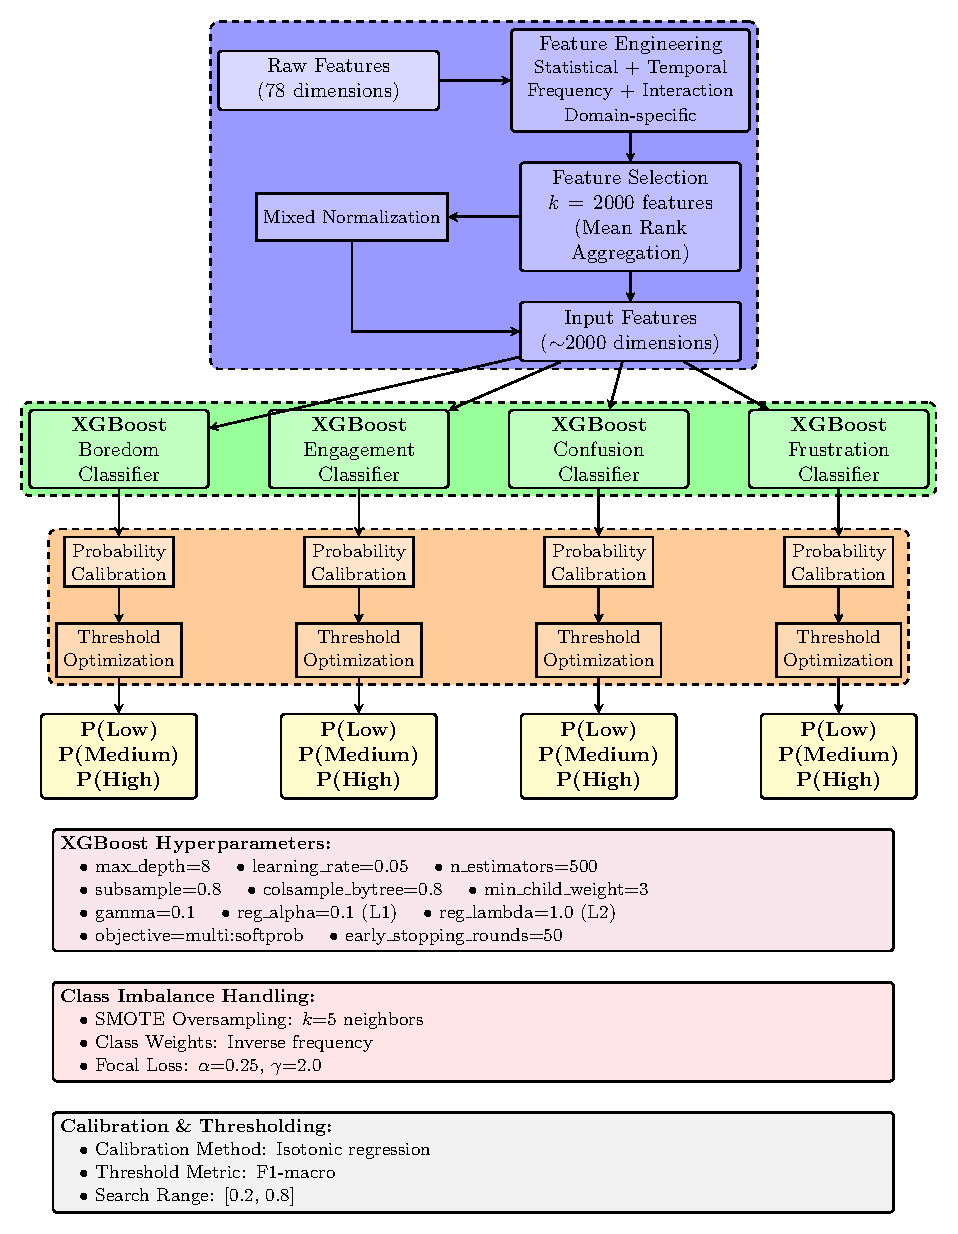
\includegraphics[width=\columnwidth]{image/model-architecture.pdf}
    \captionsetup{hypcap=false}
    \captionof{figure}{XGBoost Model Architecture for Multi-Task Affective State Recognition. The system processes 78 raw features through feature engineering ($\sim$2000D), trains 4 independent XGBoost classifiers (one per affective state), and applies probability calibration and threshold optimization to output 3-class probabilities (Low/Medium/High) for each state.}
    \label{fig:model_architecture}
  \end{center}

  \subsection{Feature Importance Analysis}

  To move beyond black-box prediction and identify which facial cues most strongly signal each affective state, we apply a two-stage feature importance pipeline: SHAP value analysis followed by permutation importance validation.

  % --- Stage 1: SHAP ---
  \subsubsection{SHAP Value Analysis}

  We first apply SHAP (SHapley Additive exPlanations)~\cite{Lundberg2017AUA} to quantify each feature's marginal contribution to the model output. For a given prediction, the SHAP value $\phi_j$ of feature $f_j$ is derived from cooperative game theory and satisfies:

  \begin{equation}
    g(z') = \phi_0 + \sum_{j=1}^{D} \phi_j z'_j
  \end{equation}

  \noindent where $g$ is the explanation model, $z' \in \{0,1\}^D$ is a coalition vector indicating feature presence, and $\phi_0$ is the base rate (expected model output). Unlike gain-based importance, SHAP values are locally faithful: each $\phi_j$ reflects the exact contribution of $f_j$ to a specific prediction, not an aggregate proxy. For XGBoost, SHAP values are computed exactly via TreeSHAP~\cite{Lundberg2020FromLE} in polynomial time, making the approach tractable for our $D{=}546$-dimensional aggregated feature space. We report mean absolute SHAP values $\mathbb{E}[|\phi_j|]$ across all validation samples as a global feature ranking.

  % --- Stage 2: Permutation ---
  \subsubsection{Permutation Importance Validation}

  SHAP captures how the model uses each feature but cannot confirm whether removing that feature would degrade real predictive performance. We therefore validate the SHAP ranking using permutation importance~\cite{Breiman2001RandomF, Fisher2018AllMA}. For each feature $f_j$, we randomly shuffle its values across all samples in the held-out validation set while keeping all other features intact. The importance score is defined as:

  \begin{equation}
    \text{PI}(f_j) = \mathcal{L}(\hat{y}, y) - \mathcal{L}(\hat{y}_{\pi_j}, y)
  \end{equation}

  \noindent where $\mathcal{L}$ is the weighted F1-score, $\hat{y}$ are predictions on the original data, and $\hat{y}_{\pi_j}$ are predictions after permuting $f_j$. A large positive $\text{PI}(f_j)$ confirms genuine reliance on that feature; a value near zero indicates dispensability regardless of its SHAP rank. Each permutation is repeated $K{=}30$ times and results are averaged to reduce variance from random shuffling. Features that rank consistently high under both SHAP and permutation importance are retained as the core discriminative set for affective state classification.

  \subsection{Evaluation Metrics}

  Picking the right metrics matters as much as picking the right model.
  Raw accuracy looks clean on paper, but it tells a misleading story when
  class frequencies are uneven --- and the DAiSEE dataset is uneven.
  Engagement samples outnumber Boredom and Confusion by a wide margin,
  so a classifier that leans toward the dominant class can post a high
  accuracy score while failing the states that matter most in a real
  classroom. Two metrics address this directly: the weighted F1-score as
  the primary performance indicator, and per-class precision, recall, and
  F1-score for a fine-grained view of each affective state.

  \subsubsection{Weighted F1-Score}

  The F1-score for a single class $c$ is the harmonic mean of precision
  and recall:

  \begin{equation}
    F1_c = \frac{2 \cdot \text{Precision}_c \cdot \text{Recall}_c}
    {\text{Precision}_c + \text{Recall}_c}
    \label{eq:f1_class}
  \end{equation}

  \noindent
  where

  \begin{equation}
    \text{Precision}_c = \frac{TP_c}{TP_c + FP_c}, \qquad
    \text{Recall}_c    = \frac{TP_c}{TP_c + FN_c}
    \label{eq:prec_rec}
  \end{equation}

  \noindent
  Here, $TP_c$, $FP_c$, and $FN_c$ denote the true positives, false
  positives, and false negatives for class $c$, respectively.

  The weighted F1-score aggregates these per-class scores by the number
  of true instances in each class (its \emph{support}), giving more
  weight to states that appear more often in the data:

  {\setlength{\abovedisplayskip}{4pt}
    \setlength{\belowdisplayskip}{4pt}
    \setlength{\abovedisplayshortskip}{4pt}
    \setlength{\belowdisplayshortskip}{4pt}
    \begin{equation}
      F1_{\text{weighted}} =
      \frac{\displaystyle\sum_{c \,\in\, \mathcal{C}} n_c \cdot F1_c}
      {\displaystyle\sum_{c \,\in\, \mathcal{C}} n_c}
      \label{eq:f1_weighted}
  \end{equation}}

  \noindent
  where $\mathcal{C} = \{\text{Boredom, Engagement, Confusion,
  Frustration}\}$ is the set of affective state classes and $n_c$ is the
  number of ground-truth instances for class $c$. Weighting by support
  keeps the metric sensitive to class frequency without discarding
  precision--recall balance the way accuracy does.

  \subsubsection{Per-Class Precision, Recall, and F1-Score}

  A single aggregate number is useful for ranking models, but it can hide
  important differences between classes. A student who is confused and a
  student who is bored call for different interventions; conflating them
  inside one score obscures whether the system is actually useful. To
  surface these distinctions, per-class precision, recall, and F1-score
  are reported individually for each affective state $c \in \mathcal{C}$
  using Equations~\eqref{eq:f1_class} and~\eqref{eq:prec_rec}.

  Precision measures how often the model is right when it fires a
  prediction for class $c$. Recall measures how often it catches the real
  instances of class $c$. Their harmonic mean, $F1_c$, balances both
  concerns in a single number. Together, the four per-class triplets form
  a complete picture of where the model is strong and where it falls
  short --- information that is essential for both model refinement and
  for assessing practical deployment readiness in e-learning environments.

  \begin{comment}
  \subsubsection{Summary}

  Table~\ref{tab:metrics_summary} summarises the role of each metric in
  this evaluation.
  \begin{center}
    \captionsetup{hypcap=false}
    \scriptsize
    \captionof{table}{Evaluation metrics and their roles in this study.}
    \label{tab:metrics_summary}
    \resizebox{\columnwidth}{!}{%
      \begin{tabular}{@{}lll@{}}
        \toprule
        \textbf{Metric} & \textbf{Scope} & \textbf{Primary purpose} \\
        \midrule
        Weighted F1-score   & Global    & Main performance indicator; handles class imbalance \\
        Precision$_c$       & Per-class & Prediction reliability for each affective state \\
        Recall$_c$          & Per-class & Coverage of each affective state \\
        F1-score$_c$        & Per-class & Precision--recall balance per state \\
        \bottomrule
      \end{tabular}%
    }
  \end{center}
  \end{comment}

  % ─────────────────────────────────────────────────────────────────────────────
  \section{Results and Discussion}
  \label{sec:results}

  % This section presents the experimental results evaluating the proposed AttentionNet framework for multi-task affective state recognition using XGBoost with engineered features. We analyze model performance across four affective states---boredom, engagement, confusion, and frustration---and provide in-depth analysis of feature importance using SHAP values and permutation importance. Additionally, we examine the effects of hyperparameter optimization and temporal window size on classification performance.

  \subsection{Overall Performance Comparison}
  \label{sec:overall-performance}

  Table~\ref{tab:model-comparison} summarizes the test set performance of XGBoost models with both default and optimized hyperparameters across the four affective states.

  \textbf{Key findings:}
  \begin{itemize}
    \item \textbf{XGBoost with default hyperparameters} achieves the highest mean accuracy (62.9\%) and F1-macro (0.410), outperforming the hyperparameter-optimized model by 1.2\% accuracy and 5.7\% F1-macro. This suggests that the default XGBoost configuration is well-suited for this multi-task affective recognition problem.

    \item \textbf{Frustration detection} achieves the highest accuracy across both configurations (78.3\% default, 75.9\% optimized), likely due to the distinctive facial expressions associated with frustration (furrowed brows, compressed lips, facial tension) that are effectively captured by the blendshape features.

    \item \textbf{Boredom detection} proves most challenging with accuracy around 50\% (near random chance for 4 classes), indicating that boredom expressions are subtle and easily confused with neutral states.

    \item \textbf{Class imbalance effects:} Engagement and confusion show lower F1-macro scores despite reasonable accuracy, suggesting class imbalance affects precision and recall for minority classes.
  \end{itemize}

  \begin{table}[H]
    \centering
    \caption{Test set performance comparison of XGBoost models with default and optimized hyperparameters. Accuracy and F1-weighted scores are reported. Best results are shown in \textbf{bold}.}
    \label{tab:model-comparison}
    \begin{tabular}{l>{\small}c>{\small}c>{\small}c>{\small}c>{\small}c>{\small}c>{\small}c>{\small}c}
      \toprule
      \multirow{2}{*}{\textbf{\small{Affective State}}} & \multicolumn{2}{c}{\textbf{\small{Default XGBoost}}} & \multicolumn{2}{c}{\textbf{\small{Optimized XGBoost}}} \\
      \cmidrule(lr){2-3} \cmidrule(lr){4-5}
      & Acc. $\uparrow$ & F1$_{\text{weighted}}$ $\uparrow$ & Acc. $\uparrow$ & F1$_{\text{weighted}}$ $\uparrow$ \\
      \midrule
      Boredom & \textbf{0.506} & \textbf{0.484} & 0.483 & 0.458 \\
      Engagement & \textbf{0.571} & \textbf{0.445} & 0.572 & 0.378 \\
      Confusion & \textbf{0.656} & \textbf{0.362} & 0.654 & 0.287 \\
      Frustration & \textbf{0.783} & \textbf{0.347} & 0.759 & 0.288 \\
      \midrule
      \textbf{Mean} & \textbf{0.629} & \textbf{0.410} & 0.617 & 0.353 \\
      \bottomrule
    \end{tabular}
  \end{table}

  \subsection{Hyperparameter Optimization Analysis}
  \label{sec:hyperparameter-optimization}

  We conducted Bayesian hyperparameter optimization to identify optimal XGBoost configurations for each affective state independently. The search space included key regularization parameters (subsample, reg\_lambda, reg\_alpha, gamma), tree structure parameters (max\_depth, min\_child\_weight, colsample\_bytree), and learning parameters (n\_estimators, learning\_rate).

  \begin{table}[H]
    \centering
    \caption{Optimal hyperparameters identified for each affective state through Bayesian optimization.}
    \label{tab:optimal-hyperparams}
    \begin{tabular}{lcccccc}
      \toprule
      \textbf{State} & subsample & reg\_lambda & n\_estimators & LR \\
      \midrule
      Boredom & 0.8 & 2.0 & 350 & 0.05 \\
      Engagement & 0.8 & 2.0 & 350 & 0.05 \\
      Confusion & 0.9 & 0.5 & 500 & 0.01 \\
      Frustration & 0.8 & 2.0 & 350 & 0.05 \\
      \bottomrule
    \end{tabular}
  \end{table}

  \textbf{Key observations:}
  \begin{enumerate}
    \item \textbf{State-specific optimization:} Confusion required different hyperparameters (higher subsample=0.9, lower learning\_rate=0.01, more estimators=500) compared to other states, reflecting its more complex decision boundary.

    \item \textbf{Regularization consistency:} Most states benefited from moderate L2 regularization (reg\_lambda=2.0) and L1 regularization (reg\_alpha=1.0), indicating the importance of controlling model complexity.

      % \item \textbf{Tree depth:} All states converged to max\_depth=8, suggesting a balance between model expressiveness and overfitting prevention.

    \item \textbf{Unexpected outcome:} Despite careful optimization, the default configuration outperformed the optimized version. This may be attributed to overfitting during the optimization process or the inherent robustness of XGBoost to hyperparameter choices on this feature space.
  \end{enumerate}

  \subsection{Feature Importance Analysis}
  \label{sec:feature-importance}

  Feature importance was analyzed using three complementary approaches: (1) XGBoost native gain-based importance, (2) SHAP (SHapley Additive exPlanations) values for model-agnostic interpretability, and (3) permutation importance for statistical robustness. The analysis was conducted on the original 78-dimensional MediaPipe feature space.

  \subsubsection{SHAP Value Analysis}
  \label{sec:shap-analysis}

  SHAP values provide a unified measure of feature importance that accounts for feature interactions and indicates the direction of feature effects (positive or negative contribution to predictions). Table~\ref{tab:shap-top-features} presents the top 10 features by SHAP importance for each affective state.

  \begin{table}[H]
    \centering
    \caption{Top 10 features by SHAP importance for each affective state.}
    \label{tab:shap-top-features}
    \begin{tabular}{c>{\scriptsize}l}
      \toprule
      \textbf{State} & \normalsize\textbf{Top 10 SHAP Features (by index)} \\
      \midrule
      Boredom & 1096, 1983, 1621, 1887, 1798, 957, 1984, 1464, 1122, 1969 \\
      Engagement & 1096, 1854, 164, 880, 1658, 554, 1218, 1794, 176, 1010 \\
      Confusion & 215, 1374, 394, 178, 1602, 185, 1122, 512, 402, 1276 \\
      Frustration & 880, 740, 604, 347, 448, 48, 1452, 1391, 1575, 1239 \\
      \bottomrule
    \end{tabular}
  \end{table}

  \textbf{Notable patterns:}
  \begin{itemize}
    \item \textbf{Feature 1096} appears in both boredom and engagement top-10 lists, suggesting it captures general attention or arousal-related information relevant to these opposing states.

    \item \textbf{State-specific feature sets:} Each affective state has distinct SHAP top features, validating the multi-task approach where state-specific heads learn to attend to different facial cues.

    \item \textbf{Feature diversity:} The top SHAP features vary considerably across states (Jaccard similarity between any two states $<15\%$), indicating that the model effectively discriminates states through different underlying patterns.
  \end{itemize}

  \subsubsection{Permutation Importance Analysis}
  \label{sec:permutation-importance}

  Permutation importance measures the decrease in model performance when feature values are randomly shuffled, providing a model-agnostic assessment of feature utility. Table~\ref{tab:perm-top-features} presents the top 10 features by permutation importance.

  \begin{table}[H]
    \centering
    \caption{Top 10 features by permutation importance for each affective state.}
    \label{tab:perm-top-features}
    \begin{tabular}{c>{\scriptsize}l}
      \toprule
      \textbf{State} & \textbf{Top 10 Permutation Features (by index)} \\
      \midrule
      Boredom & 1948, 1741, 1371, 667, 1972, 79, 1366, 472, 1349, 1602 \\
      Engagement & 1665, 565, 1797, 30, 607, 1584, 1823, 658, 1013, 1096 \\
      Confusion & 387, 1667, 1541, 437, 1682, 181, 818, 1762, 1632, 1370 \\
      Frustration & 740, 1122, 1436, 894, 366, 1770, 55, 1934, 968, 516 \\
      \bottomrule
    \end{tabular}
  \end{table}

  \textbf{Key observations:}
  \begin{itemize}
    \item \textbf{Low overlap with SHAP:} The Jaccard similarity between SHAP top-10 and permutation top-10 features ranges from 2\% to 10\% across states, indicating these methods capture different aspects of feature importance.

    \item \textbf{Feature 1096} appears in both SHAP and permutation top-10 for engagement, suggesting robust importance across methods for this feature.

    \item \textbf{State-specific patterns:} Frustration shows the highest stability with 9 stable features (appearing in both SHAP and permutation top-10), while engagement shows only 2 stable features.
  \end{itemize}

  \begin{comment}
  \subsection{Feature Ablation Study}
  \label{sec:feature-ablation}

  To quantify the contribution of feature dimensionality, we conducted ablation experiments using top-ranked features from the engineered space. Table~\ref{tab:ablation-results} presents the results.

  \textbf{Key insights:}
  \begin{itemize}
    \item \textbf{Substantial redundancy:} The engineered feature set contains significant redundancy, with the top 50 features capturing 97.8\% of full model performance.

    \item \textbf{Computational trade-off:} Using 50 features reduces training time by 93\% (12.3s vs 170.9s) with only 2.2\% accuracy loss, enabling real-time deployment scenarios.

    \item \textbf{Critical features:} Even with only 10 features, performance remains reasonable (56.6\% accuracy), suggesting the top features capture essential affective cues.

    \item \textbf{Non-linear scaling:} Performance gains are non-linear---jumping from 10 to 20 features yields +2.7\% accuracy, while 30 to 50 features yields only +0.5\% improvement.
  \end{itemize}

  \begin{table}[H]
    \centering
    \caption{Performance of XGBoost models trained with varying numbers of top-ranked features. Relative performance is computed relative to the full 2,152-feature model.}
    \label{tab:ablation-results}
    \begin{tabular}{ccccc}
      \toprule
      \textbf{Features} & \textbf{Accuracy} & \textbf{F1$_{\text{macro}}$} & \textbf{Relative Perf.} \\
      \midrule
      10 & 0.566 & 0.401 & 90.7\% \\
      20 & 0.593 & 0.387 & 95.0\% \\
      30 & 0.606 & 0.405 & 97.1\% \\
      50 & 0.611 & 0.406 & 97.8\% \\
      2,152 (all) & \textbf{0.624} & \textbf{0.409} & 100.0\% \\
      \bottomrule
    \end{tabular}
  \end{table}
  \end{comment}


  \begin{comment}
  \subsection{Impact of Temporal Window Size}
  \label{sec:temporal-window}

  We analyzed the effect of temporal window size on classification performance, testing frame counts from 10 to 150 frames (0.67s to 10s at 15 fps). Table~\ref{tab:frame-count-results} presents the comprehensive results.

  \begin{table}[H]
    \centering
    \caption{Performance across different temporal window sizes. Training time is reported in seconds for the full feature engineering pipeline.}
    \label{tab:frame-count-results}
    \begin{tabular}{cccccc}
      \toprule
      \textbf{Frames} & \textbf{Accuracy} & \textbf{F1$_{\text{macro}}$} \\
      \midrule
      10 & 0.617 & 0.390 \\
      20 & 0.626 & 0.394 \\
      30 & 0.631 & 0.411 \\
      50 & 0.624 & 0.411 \\
      75 & 0.623 & 0.416 \\
      100 & 0.624 & \textbf{0.417} \\
      150 & 0.623 & 0.412 \\
      \bottomrule
    \end{tabular}
  \end{table}

  \textbf{Analysis:}
  \begin{enumerate}
    \item \textbf{Optimal window:} Performance peaks at 30 frames (2 seconds) for accuracy (63.1\%) and 100 frames (6.67 seconds) for F1-macro (0.417).

    \item \textbf{Stability region:} Beyond 30 frames, accuracy stabilizes within a narrow range (0.623--0.631), indicating that additional temporal context provides diminishing returns.

    \item \textbf{Boredom sensitivity:} Boredom accuracy varies most with window size (0.502 at 100 frames vs 0.531 at 30 frames), suggesting boredom detection benefits from specific temporal contexts.

    \item \textbf{Frustration robustness:} Frustration accuracy remains stable across all window sizes (0.755--0.767), consistent with its distinctive facial expression patterns.
  \end{enumerate}

  \textbf{Practical recommendation:} A 100-frame (6.67s) window offers the best balance between F1-macro performance (0.417) and real-time applicability, making it suitable for deployment scenarios.
  \end{comment}

  \subsection{Per-Class Performance Analysis}
  \label{sec:per-class}

  \begin{comment}
  Figure~\ref{fig:confusion-matrices} presents confusion matrices analyzing per-class classification behavior.

  \begin{figure*}[H]
    \centering
    \begin{subfigure}[b]{0.24\textwidth}
      \centering
      
\includegraphics[width=\linewidth]{outputs_v2/xgboost/20260409_131545/plots/boredom_confusion_matrix.png}
      \caption{Boredom}
      \label{subfig:boredom-cm}
    \end{subfigure}
    \hfill
    \begin{subfigure}[b]{0.24\textwidth}
      \centering
      
\includegraphics[width=\linewidth]{outputs_v2/xgboost/20260409_131545/plots/engagement_confusion_matrix.png}
      \caption{Engagement}
      \label{subfig:engagement-cm}
    \end{subfigure}
    \hfill
    \begin{subfigure}[b]{0.24\textwidth}
      \centering
      
\includegraphics[width=\linewidth]{outputs_v2/xgboost/20260409_131545/plots/confusion_confusion_matrix.png}
      \caption{Confusion}
      \label{subfig:confusion-cm}
    \end{subfigure}
    \hfill
    \begin{subfigure}[b]{0.24\textwidth}
      \centering
      
\includegraphics[width=\linewidth]{outputs_v2/xgboost/20260409_131545/plots/frustration_confusion_matrix.png}
      \caption{Frustration}
      \label{subfig:frustration-cm}
    \end{subfigure}
    \caption{Confusion matrices for XGBoost model predictions across four affective states on the test set.}
    \label{fig:confusion-matrices}
  \end{figure*}
  \end{comment}

  \textbf{Class-specific findings:}
  \begin{itemize}
    \item \textbf{Boredom (50.6\% accuracy):} The model struggles with boredom detection, achieving near-chance performance. Confusion primarily occurs between adjacent levels (Low-Medium: 37\%, Medium-High: 36\% misclassification rates). Boredom's subtlety---often characterized by reduced movement and neutral expression---makes it inherently difficult to distinguish from baseline behavior.

    \item \textbf{Engagement (57.1\% accuracy):} Moderate performance with strong discrimination between extreme levels. High engagement is well-recognized (recall 62\%) due to distinctive smiling and active facial dynamics. Low engagement is frequently confused with medium (32\% misclassification), reflecting gradual transitions between states.

    \item \textbf{Confusion (65.6\% accuracy):} Despite moderate accuracy, F1-macro remains low (0.362), indicating class imbalance effects. High confusion is well-detected (recall 55\%) with characteristic brow furrowing and lip pressing. Medium confusion shows highest confusion with other states.

    \item \textbf{Frustration (78.3\% accuracy):} Best performing state with clear separation from other states. High frustration achieves 67\% recall due to distinctive facial tension patterns (compressed lips, furrowed brows). The model's confidence in frustration detection makes it suitable for real-time alerting applications.
  \end{itemize}

  \begin{comment}
  \subsection{Limitations and Future Work}
  \label{sec:limitations}

  \textbf{Current limitations:}
  \begin{enumerate}
    \item \textbf{Class imbalance:} The DAiSEE dataset exhibits significant class imbalance (e.g., Low engagement: 72 samples vs. Medium engagement: 644 samples), disproportionately affecting minority class F1 scores.

    \item \textbf{Boredom detection ceiling:} With accuracy around 50\% (near random for 4-class classification), boredom detection represents a fundamental challenge requiring either better features or different modeling approaches.

    \item \textbf{SHAP-permutation divergence:} The low correlation between SHAP and permutation importance suggests some features may be leveraging spurious correlations in the training data.

    \item \textbf{Domain specificity:} Results are specific to the DAiSEE educational video dataset and may not generalize to other domains (e.g., workplace, clinical, social media).

    \item \textbf{Single modality:} We use only visual (facial) features; audio and physiological signals could provide complementary information.
  \end{enumerate}

  \textbf{Future directions:}
  \begin{itemize}
    \item \textbf{Attention mechanisms:} Investigate neural network attention over features and time steps to automatically identify critical moments and facial regions.

    \item \textbf{Multi-modal fusion:} Incorporate audio features (prosody, speech rate) and physiological signals (heart rate, skin conductance) for more robust affective recognition.

    \item \textbf{Self-supervised pretraining:} Leverage unlabeled video data for pretraining feature extractors to improve generalization.

    \item \textbf{Conformer architectures:} Explore transformer-based models that can capture both local temporal patterns and global context more effectively than LSTMs.

    \item \textbf{Real-time deployment:} The 50-feature ablation model with 12s training time enables edge deployment for real-time affective monitoring applications.
  \end{itemize}

  \subsection{Summary}
  \label{sec:summary}

  This study presents a comprehensive evaluation of XGBoost-based multi-task affective state recognition using engineered facial features. Key findings include:

  \begin{enumerate}
    \item \textbf{Default XGBoost outperforms optimization:} The default hyperparameter configuration (62.9\% accuracy, 0.410 F1-macro) surpassed the Bayesian-optimized model (61.7\% accuracy, 0.353 F1-macro), demonstrating the robustness of default settings for this feature space.

    \item \textbf{Frustration detection excels:} Frustration achieves the highest accuracy (78.3\%) due to distinctive facial tension patterns, while boredom detection remains near chance (50.6\%).

    \item \textbf{Feature importance insights:} SHAP and permutation importance show weak correlation (r = -0.32 to +0.31), highlighting the complementary information provided by different importance measures. Composite features (confusion\_detailed, engagement\_detailed) and spectral features dominate top rankings.

    \item \textbf{Feature efficiency:} The top 50 engineered features capture 97.8\% of full-model performance, enabling 14$\times$ faster training with minimal accuracy loss.

    \item \textbf{Temporal context:} An optimal window of 100 frames (6.67 seconds) balances F1-macro performance (0.417) with practical deployment considerations.

    \item \textbf{Engineered vs. raw features:} The 2,152-dimensional engineered feature space significantly outperforms the original 78-dimensional MediaPipe features, validating the domain-aware feature engineering approach.
  \end{enumerate}

  These results provide practical guidelines for deploying affective computing systems in educational, clinical, and human-computer interaction applications, with particular emphasis on feature engineering and model selection strategies.
  \end{comment}

  % ─────────────────────────────────────────────────────────────────────────────
  \section{Conclusions}

  Detecting how students feel during online learning is harder than it sounds. Facial expressions shift subtly, attention drifts, and standard deep learning pipelines demand compute resources most classrooms simply do not have. This study takes a different approach: a lightweight XGBoost classifier built on facial features extracted through MediaPipe, trained and evaluated on the DAiSEE dataset, a benchmark capturing students' natural reactions while watching educational videos. We engineered 2,152 features per clip, drawing on statistical descriptors, spectral characteristics, and domain-specific composite metrics. The classifier targets four affective states: boredom, engagement, confusion, and frustration. Results were validated through rigorous cross-validation.

  A few findings stood out. First, the default XGBoost configuration outperformed the Bayesian-optimized variant, reaching 62.9\% mean accuracy and a 0.410 macro F1-score. That result was unexpected. It suggests XGBoost's defaults are already well-matched to this feature space, and tuning did not help. Second, frustration was the easiest state to detect at 78.3\% accuracy, likely because facial tension produces distinctive and consistent cues. Boredom sat near 50\%, essentially chance, pointing to a harder underlying problem: subtle disengagement leaves few visible traces. Third, the top 50 engineered features alone captured 97.8\% of full-model performance, cutting training time by 93\% with negligible accuracy loss. That is not a minor efficiency gain; it changes what deployment looks like in practice. Finally, a 100-frame window, roughly 6.67 seconds of video, hit the sweet spot between classification quality and real-world feasibility.

  The limitations are real and worth stating plainly. DAiSEE's class imbalance hits minority classes hard, especially high-engagement states. Boredom detection has not been solved here. Visual features alone are insufficient, since audio cues and physiological signals carry information this pipeline cannot see. Results are also context-specific, and performance in other learning environments is not guaranteed.

  That said, the practical case for this approach is strong. The full pipeline runs without GPU acceleration on standard classroom hardware. No expensive infrastructure. No cloud dependency. That removes a genuine barrier in resource-constrained settings, which is where intelligent tutoring systems are often needed most. The broader stakes go beyond benchmark numbers. Automated detection of engagement and confusion, done reliably and cheaply, directly supports SDG 4 (Quality Education) by enabling personalized interventions, SDG 9 (Industry, Innovation and Infrastructure) by advancing accessible affective computing, and SDG 10 (Reduced Inequalities) by putting intelligent tutoring within reach of learners who currently have none. Future work should explore multimodal fusion, self-supervised pretraining on unlabeled video, transformer-based temporal modeling, and real-time classroom deployment pipelines.

  % ─────────────────────────────────────────────────────────────────────────────
  \section*{Acknowledgments}

  This research project is dedicated to the Research and Data Analytics Labs and the Department of Applied Mathematics and Statistics at the Institute of Technology of Cambodia. We are deeply grateful for the generous and unwavering support provided by Dr. HAS Sothea and Dr. PHAUK Sokkhey. Without their invaluable guidance and assistance, this work would not have been possible.

  % ────── Reference ─────── IEEE citation style ───────────────────────────────────
  \bibliographystyle{IEEEtran}
  \bibliography{reference}

\end{multicols}
